\documentclass[11pt]{article}

\usepackage[margin=1in]{geometry}
\usepackage{graphicx}
\usepackage{tikz}
\usepackage{amsmath}
\usepackage{amssymb}
\usepackage{booktabs}
\usepackage{array}
\usepackage{listings}
\usepackage{xcolor}
\usepackage{hyperref}
\usepackage{titlesec}
\usepackage{caption}

\usetikzlibrary{shapes.geometric, arrows.meta, positioning, fit, backgrounds, calc}

\hypersetup{
  colorlinks=true,
  linkcolor=blue!50!black,
  urlcolor=blue!50!black
}

\lstset{
  basicstyle=\ttfamily\footnotesize,
  breaklines=true,
  frame=single,
  xleftmargin=1em,
  xrightmargin=1em,
  columns=flexible,
  showstringspaces=false
}

\title{Design Document: Hardware-Accelerated Block Game}
\author{Josh Bernheisel (jcb2301) \\ Wesley Maa (wm2505) \\ Mihir Joshi (mnj2122) \\[0.5em]
CSEE 4840 Embedded System Design}
\date{Spring 2026}

\begin{document}

\maketitle

\tableofcontents
\vspace{1em}
\hrule
\vspace{1em}

\section{Introduction}

We are building a hardware-accelerated 3D rendering engine on the DE1-SoC that produces a real-time, interactive block game on a VGA display. The player moves a first-person camera through a small procedurally generated world of textured cubes and can place or destroy blocks in real time.

The system partitions work between the ARM Cortex-A9 (running Linux) and custom FPGA logic. The ARM handles all control-heavy, branch-heavy computation: world representation, visibility determination, camera and matrix math, and per-quad rasterizer setup. The FPGA implements a fixed-function quadrilateral rasterizer with z-buffering, texture lookup, and VGA output generation, which is the massively parallel, arithmetic-regular part of the pipeline where custom hardware is most beneficial. A Linux kernel device driver mediates between the user-space game and the FPGA through the HPS-to-FPGA lightweight bridge.

Every face in a block world is a rectangle, so we rasterize \textbf{quadrilaterals} directly rather than tessellating into triangles. Under perspective projection, a world-space rectangle becomes a convex quadrilateral in screen space (assuming no vertex is behind the near plane, \S\ref{sec:geom}), which the four-edge-function test handles correctly. For v1 we emit one quad per exposed block face; greedy meshing to merge coplanar adjacent faces into larger rectangles is a natural optimization but is deferred past the first submitted milestone.

\textbf{Target output:} 320$\times$240 internal resolution, 8-bit palette-indexed color, double-buffered, upscaled 2$\times$2 to standard 640$\times$480 VGA timing. This resolution fits comfortably in on-chip block RAM, eliminating the need for an SDRAM controller and giving the rasterizer deterministic single-cycle access to memory.

\section{System Block Diagram}

\subsection{Top-Level View}

At the coarsest level the system is three things on the DE1-SoC board plus two external devices: the ARM HPS running Linux, a single custom FPGA peripheral (\texttt{voxel\_gpu}), and the on-board ADV7123 VGA DAC feeding the monitor. A USB keyboard and mouse attach to the HPS USB host controller; the HPS talks to \texttt{voxel\_gpu} exclusively through the lightweight HPS-to-FPGA bridge.

\begin{figure}[!htbp]
\centering
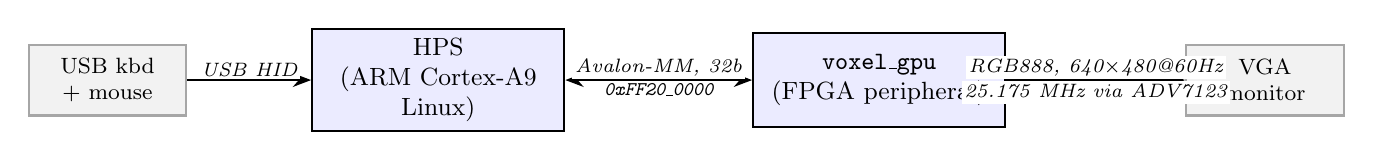
\begin{tikzpicture}[
  x=1.4cm, y=1.0cm,
  tlblock/.style={rectangle, draw, thick, minimum width=3.2cm, minimum height=1.2cm,
                  align=center, font=\small, fill=blue!8},
  extblock/.style={rectangle, draw=gray!70, fill=gray!10, thick,
                   minimum width=2.0cm, minimum height=0.9cm, align=center, font=\footnotesize},
  arrow/.style={-Stealth, thick},
  biarrow/.style={Stealth-Stealth, thick},
  elbl/.style={font=\scriptsize\itshape, fill=white, inner sep=1pt}
]
\node[extblock] (usb) at (0, 2) {USB kbd\\+ mouse};
\node[tlblock]  (hps) at (3, 2) {HPS\\(ARM Cortex-A9\\Linux)};
\node[tlblock]  (vgpu) at (7, 2) {\texttt{voxel\_gpu}\\(FPGA peripheral)};
\node[extblock] (vga) at (10.5, 2) {VGA\\monitor};

\draw[arrow] (usb) -- node[elbl,above]{USB HID} (hps);
\draw[biarrow] (hps) -- node[elbl,above]{Avalon-MM, 32b}
                       node[elbl,below]{\texttt{0xFF20\_0000}} (vgpu);
\draw[arrow] (vgpu) -- node[elbl,above]{RGB888, 640$\times$480@60Hz}
                       node[elbl,below]{25.175~MHz via ADV7123} (vga);
\end{tikzpicture}
\caption{Top-level view. The dashed region in Figure~\ref{fig:blockdiagram} expands the \texttt{voxel\_gpu} peripheral and the software stack running on the HPS.}
\label{fig:toplevel}
\end{figure}

\subsection{Internal Block Diagram}

The \texttt{voxel\_gpu} peripheral and the software stack on the HPS together comprise twelve major functional blocks split across software (user-space C on Linux, blocks~1--5), a kernel driver (block~6), and hardware (SystemVerilog on the FPGA fabric, blocks~7--12).

\begin{figure}[!htbp]
\centering
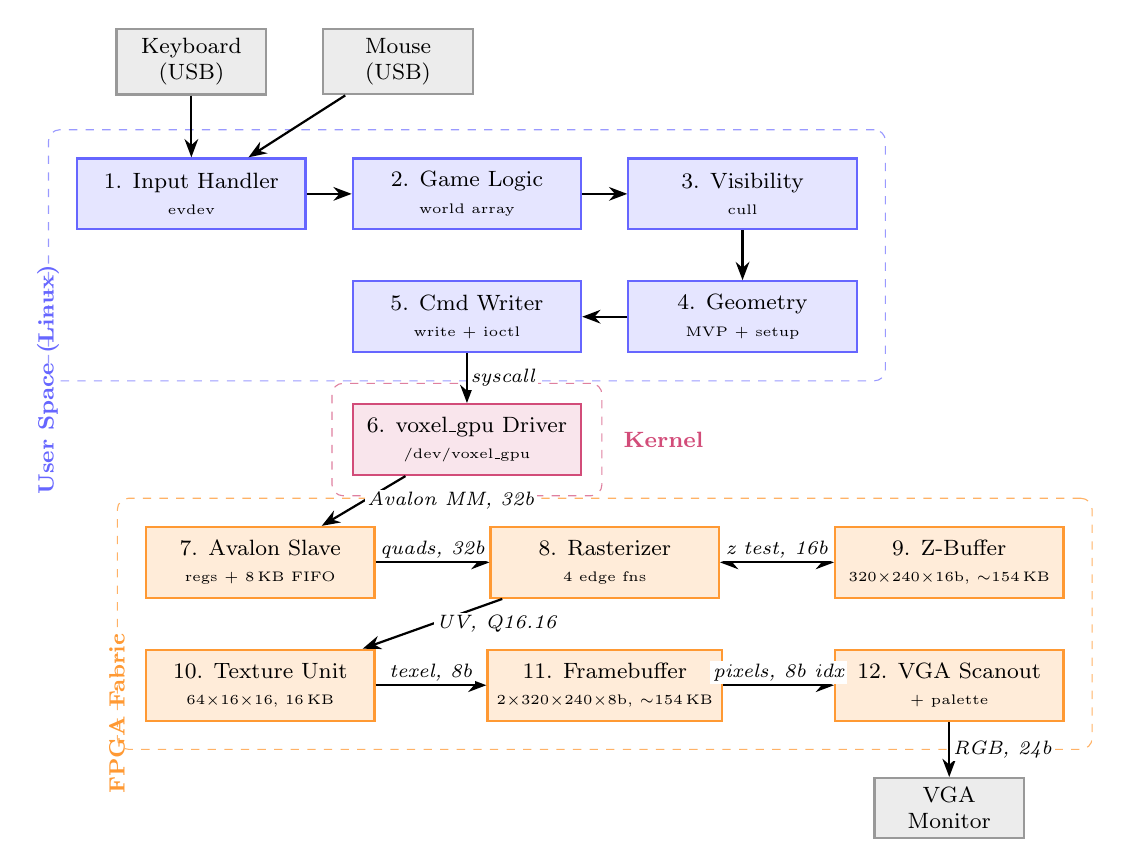
\begin{tikzpicture}[
  x=1.75cm, y=1.2cm,
  swblock/.style={rectangle, draw=blue!60, fill=blue!10, thick,
                  minimum width=2.9cm, minimum height=0.9cm, align=center,
                  font=\footnotesize},
  kernblock/.style={rectangle, draw=purple!70, fill=purple!10, thick,
                    minimum width=2.9cm, minimum height=0.9cm, align=center,
                    font=\footnotesize},
  hwblock/.style={rectangle, draw=orange!80, fill=orange!15, thick,
                  minimum width=2.9cm, minimum height=0.9cm, align=center,
                  font=\footnotesize},
  extblock/.style={rectangle, draw=gray!80, fill=gray!15, thick,
                   minimum width=1.9cm, minimum height=0.75cm, align=center,
                   font=\footnotesize},
  arrow/.style={-Stealth, thick},
  biarrow/.style={Stealth-Stealth, thick},
  elbl/.style={font=\scriptsize\itshape, fill=white, inner sep=1pt}
]

% Row Y=7: External input
\node[extblock] (kbd)   at (0.5, 7) {Keyboard\\(USB)};
\node[extblock] (mouse) at (2.0, 7) {Mouse\\(USB)};

% Row Y=5.6: Software row A (input -> game -> visibility)
\node[swblock] (input) at (0.5, 5.6) {1. Input Handler\\\tiny{evdev}};
\node[swblock] (game)  at (2.5, 5.6) {2. Game Logic\\\tiny{world array}};
\node[swblock] (vis)   at (4.5, 5.6) {3. Visibility\\\tiny{cull}};

% Row Y=4.3: Software row B (cmdw <- geometry)
\node[swblock] (cmdw) at (2.5, 4.3) {5. Cmd Writer\\\tiny{write + ioctl}};
\node[swblock] (geom) at (4.5, 4.3) {4. Geometry\\\tiny{MVP + setup}};

% Row Y=3.0: Kernel
\node[kernblock] (drv) at (2.5, 3.0) {6. voxel\_gpu Driver\\\tiny{/dev/voxel\_gpu}};

% Row Y=1.7: Hardware row A
\node[hwblock] (avalon) at (1.0, 1.7) {7. Avalon Slave\\\tiny{regs + 8\,KB FIFO}};
\node[hwblock] (rast)   at (3.5, 1.7) {8. Rasterizer\\\tiny{4 edge fns}};
\node[hwblock] (zbuf)   at (6.0, 1.7) {9. Z-Buffer\\\tiny{320$\times$240$\times$16b, $\sim$154\,KB}};

% Row Y=0.4: Hardware row B
\node[hwblock] (tex) at (1.0, 0.4) {10. Texture Unit\\\tiny{64$\times$16$\times$16, 16\,KB}};
\node[hwblock] (fb)  at (3.5, 0.4) {11. Framebuffer\\\tiny{2$\times$320$\times$240$\times$8b, $\sim$154\,KB}};
\node[hwblock] (vga) at (6.0, 0.4) {12. VGA Scanout\\\tiny{+ palette}};

% Row Y=-0.9: Monitor
\node[extblock] (mon) at (6.0, -0.9) {VGA\\Monitor};

% Background groupings (drawn behind)
\begin{pgfonlayer}{background}
  \node[fit=(input) (game) (vis) (geom) (cmdw), draw=blue!40, dashed,
        inner sep=0.35cm, rounded corners,
        label={[blue!60, font=\footnotesize\bfseries, rotate=90]left:User Space (Linux)}] {};
  \node[fit=(drv), draw=purple!50, dashed, inner sep=0.25cm, rounded corners] {};
  \node[fit=(avalon) (rast) (zbuf) (tex) (fb) (vga), draw=orange!60, dashed,
        inner sep=0.35cm, rounded corners,
        label={[orange!80, font=\footnotesize\bfseries, rotate=90]left:FPGA Fabric}] {};
\end{pgfonlayer}

% Kernel label on right side
\node[purple!70, font=\footnotesize\bfseries, right=0.4cm of drv] {Kernel};

% --- Arrows ---
% Input devices into input handler
\draw[arrow] (kbd)   -- (input);
\draw[arrow] (mouse) -- (input);

% Software pipeline (top row, left to right)
\draw[arrow] (input) -- (game);
\draw[arrow] (game)  -- (vis);

% Visibility -> Geometry (down)
\draw[arrow] (vis) -- (geom);

% Geometry -> Cmd Writer (right to left)
\draw[arrow] (geom) -- (cmdw);

% Cmd Writer -> Driver (down)
\draw[arrow] (cmdw) -- node[elbl,right]{syscall} (drv);

% Driver -> Avalon Slave
\draw[arrow] (drv) -- node[elbl,right]{Avalon MM, 32b} (avalon);

% Hardware: Avalon -> Rasterizer
\draw[arrow] (avalon) -- node[elbl,above]{quads, 32b} (rast);

% Rasterizer <-> Z-Buffer
\draw[biarrow] (rast) -- node[elbl,above]{z test, 16b} (zbuf);

% Rasterizer -> Texture (down-left)
\draw[arrow] (rast) -- node[elbl,right]{UV, Q16.16} (tex);

% Texture -> Framebuffer (right along bottom row)
\draw[arrow] (tex) -- node[elbl,above]{texel, 8b} (fb);

% Framebuffer -> VGA Scanout
\draw[arrow] (fb) -- node[elbl,above]{pixels, 8b idx} (vga);

% VGA -> Monitor
\draw[arrow] (vga) -- node[elbl,right]{RGB, 24b} (mon);

\end{tikzpicture}
\caption{System block diagram. Data flows from USB input, through the Linux game on the ARM, across the Avalon bus via a kernel driver, into the FPGA rasterizer pipeline, and out to the VGA monitor. Dashed regions separate user-space software, kernel-space driver, and FPGA fabric.}
\label{fig:blockdiagram}
\end{figure}

\subsection{Block Descriptions}

\textbf{Software blocks (user space, running on ARM Cortex-A9 under Linux):}

\begin{enumerate}
\item \textbf{Input Handler}: Reads USB keyboard and mouse events from \texttt{/dev/input/event*} using the Linux evdev API, which surfaces decoded USB HID reports as \texttt{struct input\_event}\,\{\texttt{timeval}, \texttt{type}, \texttt{code}, \texttt{value}\} records. Concretely, a USB boot-protocol mouse produces 3-byte reports of $\{\text{buttons}, dx, dy\}$ at $\sim$125~Hz, which the kernel HID layer decodes into \texttt{EV\_REL}/\texttt{REL\_X}/\texttt{REL\_Y} events; a boot keyboard produces 8-byte reports (modifier mask plus up to six keycodes) that surface as \texttt{EV\_KEY}. Our handler accumulates these between frames and produces camera deltas (yaw, pitch, translation) and block place/destroy events each frame.

\item \textbf{Game Logic}: Maintains world state as 16$\times$16$\times$16 chunks of block IDs. Processes player actions and updates the world array in place.

\item \textbf{Visibility Stage}: Performs view-frustum culling on chunks (tests chunk AABB against six frustum planes), then hidden-face culling on blocks within visible chunks. Emits a list of visible quads.

\item \textbf{Geometry Stage}: Transforms each quad's four vertices through the combined model-view-projection matrix (Q16.16 fixed-point), performs perspective divide and viewport mapping. Computes edge-function coefficients $(A_i, B_i, C_i)$, depth gradients, and UV gradients for each quad.

\item \textbf{Command Buffer Writer}: Writes quad descriptors to the shared FIFO region via \texttt{write()} on \texttt{/dev/voxel\_gpu}, then issues an ioctl to flip buffers.
\end{enumerate}

\textbf{Kernel-space block:}

\begin{enumerate}
\setcounter{enumi}{5}
\item \textbf{voxel\_gpu Device Driver}: Platform driver bound to \texttt{csee4840,voxel\_gpu-1.0}. Maps the FPGA's lightweight bridge registers, exposes \texttt{/dev/voxel\_gpu}, and implements ioctls for palette upload, frame submission, and status query.
\end{enumerate}

\textbf{Hardware blocks (FPGA fabric):}

\begin{enumerate}
\setcounter{enumi}{6}
\item \textbf{Avalon MM Slave}: Receives 32-bit writes from the ARM to control registers and to the memory-mapped command FIFO window. Exposes status registers back.

\item \textbf{Quad Rasterizer}: Pops quad descriptors from the command FIFO, iterates each quad's bounding box, evaluates four edge functions per pixel, interpolates depth and UV coordinates incrementally.

\item \textbf{Z-Buffer Unit}: 16-bit depth buffer at 320$\times$240 in BRAM ($\sim$154~KB). Compares interpolated depth against stored depth; gates framebuffer writes.

\item \textbf{Texture Unit}: Stores up to 64 16$\times$16 palette-indexed texture tiles in BRAM. Nearest-neighbor UV lookup.

\item \textbf{Framebuffer}: Double-buffered 320$\times$240 8bpp framebuffers in BRAM.

\item \textbf{VGA Scanout + Palette}: VGA timing controller reads the front buffer, looks up RGB888 values through a 256-entry palette BRAM, and drives the on-board ADV7123 DAC at 640$\times$480@60Hz with 2$\times$2 pixel doubling.
\end{enumerate}

\subsection{Communication Pathways}

\begin{itemize}
\item \textbf{USB $\rightarrow$ Linux $\rightarrow$ Input Handler}: HID events polled per frame via evdev.
\item \textbf{Game Logic $\leftrightarrow$ Visibility $\leftrightarrow$ Geometry $\leftrightarrow$ Command Writer}: In-process function calls, all user-space C; data structures are 3D \texttt{uint8\_t} block arrays and \hyperref[sec:quaddesc]{\texttt{quad\_desc\_t}} structs.
\item \textbf{User space $\rightarrow$ Driver}: \texttt{write()} for bulk command stream data, \texttt{ioctl()} for control (palette, flip, status). Driver uses \texttt{copy\_from\_user} then \texttt{iowrite32} across the bridge.
\item \textbf{Driver $\rightarrow$ Avalon MM Slave}: 32-bit writes over the HPS-to-FPGA lightweight bridge at base \texttt{0xFF20\_0000}.
\item \textbf{Avalon Slave $\rightarrow$ Rasterizer}: 8~KB command FIFO in BRAM; ARM pushes descriptors, rasterizer pops them.
\item \textbf{Rasterizer $\rightarrow$ Z-buffer / Framebuffer}: Direct M10K BRAM ports sustaining one pixel per cycle. The Z-buffer uses a dual-port pipelined read-modify-write (read at cycle $n$, conditional write at cycle $n{+}1$); the framebuffer back buffer uses a write port while scanout reads the front buffer on the opposite port (see \S\ref{sec:rast}).
\item \textbf{Framebuffer $\rightarrow$ Scanout $\rightarrow$ Palette $\rightarrow$ DAC}: Three-stage pipeline at the 25.175~MHz VGA pixel clock.
\end{itemize}

\section{Algorithms}

\subsection{Hidden-Face Culling (software)}

For each solid block in a visible chunk, check all six axis-aligned neighbors. Emit a quad for a face only if the neighbor on that side is air (or outside the chunk boundary with the adjacent chunk's neighbor block air). This eliminates interior geometry.

\begin{lstlisting}[language=C]
for each chunk C in visible_chunks:
  for each block B at (x,y,z) in C:
    if B is air: continue
    for each direction d in {+x, -x, +y, -y, +z, -z}:
      N = block_at(x,y,z + offset(d))
      if N is air:
        emit_quad(B, d)
\end{lstlisting}

\subsection{View-Frustum Culling (software)}

Before per-block work, reject entire chunks whose axis-aligned bounding boxes fall outside the camera frustum. Each chunk's 8 corners are tested against the 6 frustum planes derived from the view-projection matrix. If all 8 corners lie on the outside half-space of any single plane, the chunk is culled. Some chunks partially outside the frustum will pass, but no visible chunk is ever rejected.

\subsection{Vertex Transformation and Quad Setup (software)}
\label{sec:geom}

For each emitted quad (four vertices in world space):
\begin{enumerate}
\item Multiply each vertex by the combined model-view-projection matrix (4$\times$4, Q16.16 fixed-point).
\item \textbf{Near-plane handling.} If any of the four vertices has $w \leq w_{\text{near}}$ (with $w_{\text{near}} = 0.1$ world units, i.e.\ 10\% of a block edge), the quad straddles or lies behind the near plane; perspective divide would produce invalid (negative or enormous) screen coordinates and the projected shape may be non-convex, breaking the edge-function test. For v1 we \emph{reject} such quads outright (cheap, one comparison per vertex). The visual artifact is that a face partially behind the camera pops out of view one frame early; acceptable given a small near-plane distance. A future revision can replace rejection with Sutherland--Hodgman clipping against the near plane, which splits the quad into a convex polygon of up to five vertices --- more work for the geometry stage but no change to the rasterizer contract.
\item Perspective divide: divide $x, y, z$ by $w$.
\item Viewport map: $\text{screen}_x = (x+1) \cdot 160$, $\text{screen}_y = (1-y) \cdot 120$.
\item Compute four edge coefficients. For an edge from $(x_0, y_0)$ to $(x_1, y_1)$:
\[ A = y_0 - y_1, \quad B = x_1 - x_0, \quad C = -(A \cdot x_0 + B \cdot y_0) \]
The edge function $E(x,y) = Ax + By + C$ is non-negative on the interior side when vertices are emitted in screen-space clockwise order (equivalently, counterclockwise in NDC, before the $(1-y)$ viewport flip inverts handedness). Software packs each coefficient as signed Q24.8 (value $\cdot 256$) before writing to the descriptor; see the rationale following Table~\ref{tab:quaddesc}.
\item Compute depth plane coefficients $z(x,y) = z_0 + \frac{dz}{dx}x + \frac{dz}{dy}y$ from the three screen-space vertices with their depths.
\item Compute UV gradients for textured quads.
\item Compute the screen-space bounding box, clamped to $[0, 319] \times [0, 239]$.
\end{enumerate}

The output is one \hyperref[sec:quaddesc]{\texttt{quad\_desc\_t}} per quad, pushed to the command FIFO.

\subsection{Quad Rasterization (hardware)}
\label{sec:rast}

For each quad descriptor popped from the FIFO:

\begin{lstlisting}[language=C]
// Initialize at (x_min, y_min)
E0 = A0*x_min + B0*y_min + C0  (similarly E1, E2, E3)
z  = z0 + dz_dx*x_min + dz_dy*y_min
u, v = similarly

for y = y_min to y_max:
  save row-start values of E0..E3, z, u, v
  for x = x_min to x_max:
    if (E0 >= 0) and (E1 >= 0) and (E2 >= 0) and (E3 >= 0):
      z_cur = z_buffer[x, y]
      if z < z_cur:
        if flags.TEX:
          color_idx = texture_fetch(u, v, tex_or_color)
        else:
          color_idx = tex_or_color   // flat palette index
        framebuffer_back[x, y] = color_idx
        z_buffer[x, y] = z
    E0 += A0; E1 += A1; E2 += A2; E3 += A3
    z  += dz_dx; u += du_dx; v += dv_dx
  restore row-start; step: E_i += B_i; z += dz_dy; etc.
\end{lstlisting}

The crucial property exploited in hardware: edge functions, depth, and UV all advance by a \emph{constant} when stepping one pixel in $x$ or $y$. Per-pixel work reduces to four adds and four sign checks in the inner loop. This maps directly to a shallow pipeline.

\paragraph{BRAM port arrangement.} Each rasterized pixel touches multiple on-chip memories, but careful port assignment keeps steady-state throughput at one pixel per cycle.

\begin{itemize}
\item \textbf{Z-buffer:} read-modify-write per pixel. Implemented on a true dual-port M10K with the read port issuing the depth fetch on cycle $n$ and the write port committing the update on cycle $n+1$ --- a two-stage pipeline sustains one access per cycle. Within a single quad, consecutive pixels address distinct cells so no read-after-write hazard arises; at quad boundaries the rasterizer inserts one idle cycle while edge, depth, and UV coefficients are reloaded, which also drains any in-flight write before the next quad's first read is issued. Alternatively, a single-port BRAM clocked at 2$\times$ the rasterizer rate would serve both accesses; we prefer the dual-port approach for simpler timing closure.
\item \textbf{Framebuffer:} one write per passing pixel on the rasterizer-facing port. The opposite port belongs to the scanout pipeline. Because the design is double-buffered (the rasterizer writes the \emph{back} buffer while scanout reads the \emph{front}), there is no port contention between the two domains --- they target different BRAMs until \texttt{VGPU\_FLIP}.
\item \textbf{Texture BRAM:} one read per textured pixel. Single-port sufficient; rasterizer stalls one cycle if a simultaneous access is needed (not triggered in the current design).
\item \textbf{Frame clear (\texttt{CLR}).} A single linear sweep over the 76{,}800 pixel addresses writes both the Z-buffer (to \texttt{0xFFFF}) and the back framebuffer (to palette index 0) each cycle --- the two BRAMs have independent write ports, so both clears happen in parallel without extending the sweep. At 50~MHz this takes $\sim$1.5~ms, comfortably inside the 16.6~ms frame budget; the rasterizer stays idle via the \texttt{BSY}/\texttt{CLR} handshake until the sweep completes. Clearing the back framebuffer is necessary in v1 because there is no skybox; otherwise any pixel not covered by a rasterized quad would expose stale contents from two frames ago.
\end{itemize}

\subsection{VGA Scanout with Palette Lookup (hardware)}

A three-stage pipeline at the 25.175~MHz pixel clock:

\begin{figure}[h]
\centering
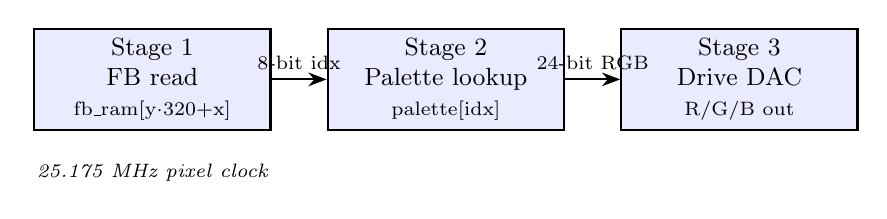
\begin{tikzpicture}[
  stage/.style={rectangle, draw, thick, minimum width=3.0cm, minimum height=1.2cm,
                align=center, font=\small, fill=blue!8},
  arrow/.style={-Stealth, thick}
]
\node[stage] (fb) at (0,0) {Stage 1\\FB read\\\scriptsize{fb\_ram[y$\cdot$320+x]}};
\node[stage, right=0.7cm of fb] (pal) {Stage 2\\Palette lookup\\\scriptsize{palette[idx]}};
\node[stage, right=0.7cm of pal] (dac) {Stage 3\\Drive DAC\\\scriptsize{R/G/B out}};

\draw[arrow] (fb) -- node[above,font=\scriptsize]{8-bit idx} (pal);
\draw[arrow] (pal) -- node[above,font=\scriptsize]{24-bit RGB} (dac);

\node[below=0.3cm of fb, font=\scriptsize\itshape] {25.175 MHz pixel clock};
\end{tikzpicture}
\caption{VGA scanout pipeline. Each stage is one cycle at the 25.175~MHz pixel clock; after priming, one pixel is driven to the DAC per clock.}
\label{fig:scanout}
\end{figure}

\paragraph{2$\times$2 pixel doubling.} The framebuffer is 320$\times$240 but VGA timing drives 640$\times$480, so the scanout address is computed as
\[
  \text{fb\_addr} = \text{hcount}[9{:}1] + 320 \cdot \text{vcount}[8{:}1],
\]
i.e., the low bit of each counter is dropped. The same address is therefore presented to the framebuffer port for two consecutive pixel clocks horizontally and on two consecutive lines vertically, so every 320$\times$240 logical pixel appears as a 2$\times$2 block at 640$\times$480. A naive implementation re-reads the framebuffer every cycle despite the address not changing; a more efficient variant latches the color and only issues BRAM reads on even \texttt{hcount}, but both produce identical output. The scanout side sees the framebuffer through its dedicated BRAM port, independent of the rasterizer side (see Z-buffer / framebuffer discussion in \S\ref{sec:rast}).

\subsection{Texture Lookup (hardware)}

Textures are 16$\times$16 palette-indexed tiles stored in BRAM. The rasterizer carries $u$ and $v$ as Q16.16 fixed-point. The full integer range is not needed for a 16$\times$16 tile --- only the low four integer bits index the texel, with higher bits masked (equivalently, $\bmod\,16$) to wrap --- but Q16.16's fractional precision ($2^{-16}$ per step) keeps accumulated interpolation error well under a texel across a full 320-pixel scan line, whereas a narrower format such as Q8.8 would drift by over one texel per row and produce visible seams. Nearest-neighbor lookup:
\[ \text{texel} = \text{tex\_ram}[\text{tex\_or\_color}][\lfloor u \rfloor \bmod 16][\lfloor v \rfloor \bmod 16] \quad (\texttt{TEX=1}) \]
The output is an 8-bit palette index, written directly to the framebuffer.

\paragraph{Affine vs.\ perspective-correct interpolation.} The UV gradients $du_{dx}, dv_{dx}, du_{dy}, dv_{dy}$ are \emph{affine} in screen space, so $u$ and $v$ advance by a constant per pixel --- the same adder-per-step scheme as the edge functions, and the reason texturing costs only two extra adds per pixel in hardware. Strictly, the correct quantities to interpolate linearly in screen space are $u/w$, $v/w$, and $1/w$, divided per pixel to recover true $u, v$; affine interpolation is an approximation that produces visible warping on quads at steep viewing angles (the classic ``PS1 look''). For a $320\times240$ viewport of block-game content, the artifact is rarely objectionable and saves one divider per pixel. \emph{Future fix:} add $1/w$, $u/w$, $v/w$ to the descriptor, pipeline a reciprocal unit (a $\sim$10-cycle Newton--Raphson iterator or a $2^{10}$-entry lookup) into the rasterizer, and divide per pixel; the rest of the pipeline is unchanged. This is a clean upgrade path once the affine version is working.

\section{Resource Budgets}

\subsection{On-chip BRAM}

The Cyclone V on the DE1-SoC has approximately 4~Mbit ($\approx$512~KB) of on-chip M10K block RAM.

\begin{table}[h]
\centering
\begin{tabular}{lrl}
\toprule
\textbf{Resource} & \textbf{Size} & \textbf{Notes} \\
\midrule
Framebuffer $\times$2 (320$\times$240, 8bpp) & 153.6~KB & Double-buffered \\
Z-buffer (320$\times$240, 16-bit) & 153.6~KB & Cleared per frame \\
Palette (256 $\times$ RGB888) & 0.75~KB & Uploaded at startup \\
Texture tiles (64 $\times$ 16$\times$16 $\times$ 8bpp) & 16~KB & Expandable \\
Quad command FIFO & 8~KB & $\sim$128 quads in flight \\
\midrule
\textbf{Total BRAM} & \textbf{$\sim$332~KB} & \textbf{$\sim$65\% of available} \\
\bottomrule
\end{tabular}
\caption{On-chip block RAM budget. Extra headroom for expansion if needed.}
\end{table}

\subsection{DDR3 (HPS side, 1 GB available)}

\begin{table}[h]
\centering
\begin{tabular}{lr}
\toprule
\textbf{Resource} & \textbf{Size} \\
\midrule
World data (up to 128 chunks loaded, 4~KB each) & $\sim$512~KB \\
Per-frame visible quad list & $<$64~KB \\
Linux kernel + user program + assets & $<$64~MB \\
\bottomrule
\end{tabular}
\caption{DDR3 usage on the HPS side; effectively unbounded relative to our needs.}
\end{table}

\subsection{Rasterizer Throughput}

At 50~MHz FPGA clock with a single-pixel-per-cycle rasterizer, theoretical peak is 50~Mpix/s. A fully-covered 320$\times$240 frame is 76{,}800 pixels = 1.5~ms of rasterizer time. At 60~fps (16.6~ms budget), we can afford $\sim$10$\times$ overdraw. Typical first-person views of voxel terrain have depth complexity in the 2--4$\times$ range after back-face and hidden-face culling, well within budget even without occlusion culling between surviving faces.

\subsection{Command Buffer Bandwidth}

Flat-shaded descriptors are 64~bytes; textured descriptors are 128~bytes (see \S\ref{sec:quaddesc}). Assuming the worst case --- every visible quad textured --- at 60~fps with $\sim$500 visible quads per frame (generous post-cull estimate): $500 \cdot 128 \cdot 60 \approx 3.84$~MB/s over the lightweight bridge, which sustains tens of MB/s. Not a bottleneck.

\section{Hardware/Software Interface}

The ARM communicates with the rasterizer through two mechanisms: a small set of \textbf{control registers} at fixed Avalon MM offsets for commands and status, and a larger \textbf{memory-mapped FIFO window} for streaming quad descriptor data.

\subsection{Control Register Map}

Base address: \texttt{0xFF20\_0000} (assigned by Platform Designer; actual value determined from the device tree). All registers are 32 bits. Addresses are byte offsets from base.

\vspace{0.5em}
\noindent\textbf{Offset 0x00: CONTROL (R/W)}
\vspace{0.3em}

\begin{center}
\begin{tabular}{|c|c|c|c|}
\hline
\texttt{[31:3]} & \texttt{[2]} & \texttt{[1]} & \texttt{[0]} \\
\hline
reserved & CLR & FLP & EN \\
\hline
\end{tabular}
\end{center}

\begin{tabular}{rlp{0.62\linewidth}}
Bit 0 & EN  & Rasterizer enable. 0 = idle, safe to reconfigure; 1 = process FIFO. \\
Bit 1 & FLP & Buffer flip request. Write 1 to swap front/back on next vsync. Auto-clears. \\
Bit 2 & CLR & Frame clear. Write 1 to launch a linear sweep that writes Z-buffer $\leftarrow$ \texttt{0xFFFF} (far) and back framebuffer $\leftarrow$ palette index 0 in parallel, one pair of writes per cycle (the two BRAMs have independent write ports). Auto-clears when the sweep completes. Both buffers must be cleared every frame since without a skybox, uncovered back-buffer pixels would otherwise show stale contents from two frames ago. \\
Bits 31:3 & --- & Reserved, write 0. \\
\end{tabular}

\vspace{0.3em}
\noindent For v1, software drives frame pacing by \emph{polling} \texttt{STATUS.FEM} (FIFO empty) and \texttt{STATUS.VSY} (vblank) rather than taking a hardware interrupt. At 60~fps the polling cost is negligible (tens of reads per 16~ms frame).

\vspace{0.8em}
\noindent\textbf{Offset 0x04: STATUS (R only)}
\vspace{0.3em}

\begin{center}
\begin{tabular}{|c|c|c|c|c|c|}
\hline
\texttt{[31:16]} & \texttt{[15:4]} & \texttt{[3]} & \texttt{[2]} & \texttt{[1]} & \texttt{[0]} \\
\hline
reserved & FIFO\_WORDS & VSY & FEM & FFL & BSY \\
\hline
\end{tabular}
\end{center}

\begin{tabular}{rlp{0.62\linewidth}}
Bit 0 & BSY & Rasterizer busy (actively processing a quad). \\
Bit 1 & FFL & Command FIFO full. Subsequent writes are back-pressured by the slave asserting Avalon \texttt{waitrequest} until a slot frees (no data is dropped); software reads FFL only as a hint to pace writes. \\
Bit 2 & FEM & Command FIFO empty. \\
Bit 3 & VSY & Currently in vertical blanking interval (safe to flip). \\
Bits 15:4 & FIFO\_WORDS & Number of 32-bit words currently queued in the command FIFO, 0--2048. \\
Bits 31:16 & --- & Reserved. \\
\end{tabular}

\vspace{0.3em}
\noindent The FIFO reports its fill level in \emph{words} rather than descriptors because the hardware cannot know descriptor boundaries at enqueue time --- a flat-shaded quad is 16 words (64 bytes) and a textured quad is 32 words (128 bytes). Software divides by 16 (or 32) as appropriate when deciding whether a push will fit.

\vspace{0.8em}
\noindent\textbf{Offset 0x08: FRAME\_COUNT (R only)} --- 32-bit counter incremented once per completed frame. Used by software for FPS measurement.

\vspace{0.5em}
\noindent\textbf{Offset 0x0C: PALETTE\_ADDR (W only)} --- palette entry index (0--255) to program next. Writing arms the palette write port.

\vspace{0.5em}
\noindent\textbf{Offset 0x10: PALETTE\_DATA (W only)}

\begin{center}
\begin{tabular}{|c|c|c|c|}
\hline
\texttt{[31:24]} & \texttt{[23:16]} & \texttt{[15:8]} & \texttt{[7:0]} \\
\hline
reserved & RED & GREEN & BLUE \\
\hline
\end{tabular}
\end{center}

Writing \texttt{PALETTE\_DATA} commits the RGB888 value to \texttt{palette[PALETTE\_ADDR]} and auto-increments \texttt{PALETTE\_ADDR}. At startup, software writes \texttt{PALETTE\_ADDR} once, then \texttt{PALETTE\_DATA} 256 times to upload the full palette.

\vspace{0.5em}
\noindent\textbf{Offsets 0x1000--0x2FFF: FIFO\_WINDOW (W only)} --- 8~KB memory-mapped window into the command FIFO. Writes are enqueued as quad descriptor data. Software writes 16 consecutive 32-bit words to push one 64-byte flat-shaded descriptor, or 32 consecutive words (128 bytes) for a textured descriptor.

\subsection{Quad Descriptor Format}
\label{sec:quaddesc}

Each descriptor is 64 bytes, written as 16 consecutive 32-bit little-endian words through \texttt{FIFO\_WINDOW}. The rasterizer pops one descriptor at a time in exactly this layout.

\begin{table}[h]
\centering
\small
\begin{tabular}{rrllp{0.36\linewidth}}
\toprule
\textbf{Offset} & \textbf{Size} & \textbf{Field} & \textbf{Format} & \textbf{Meaning} \\
\midrule
 0 & 2 & \texttt{x\_min}    & int16             & Bounding box left \\
 2 & 2 & \texttt{y\_min}    & int16             & Bounding box top \\
 4 & 2 & \texttt{x\_max}    & int16             & Bounding box right \\
 6 & 2 & \texttt{y\_max}    & int16             & Bounding box bottom \\
 8 & 4 & \texttt{edge0\_A}  & int32 Q24.8       & Edge 0 coefficient A \\
12 & 4 & \texttt{edge0\_B}  & int32 Q24.8       & Edge 0 coefficient B \\
16 & 4 & \texttt{edge0\_C}  & int32 Q24.8       & Edge 0 coefficient C \\
20 & 4 & \texttt{edge1\_A}  & int32 Q24.8       & Edge 1 A \\
24 & 4 & \texttt{edge1\_B}  & int32 Q24.8       & Edge 1 B \\
28 & 4 & \texttt{edge1\_C}  & int32 Q24.8       & Edge 1 C \\
32 & 4 & \texttt{edge2\_A}  & int32 Q24.8       & Edge 2 A \\
36 & 4 & \texttt{edge2\_B}  & int32 Q24.8       & Edge 2 B \\
40 & 4 & \texttt{edge2\_C}  & int32 Q24.8       & Edge 2 C \\
44 & 4 & \texttt{edge3\_A}  & int32 Q24.8       & Edge 3 A \\
48 & 4 & \texttt{edge3\_B}  & int32 Q24.8       & Edge 3 B \\
52 & 4 & \texttt{edge3\_C}  & int32 Q24.8       & Edge 3 C \\
56 & 2 & \texttt{z0}        & uint16 Q1.15      & Depth at $(x_{\min}, y_{\min})$; range $[0,\,2)$ \\
58 & 2 & \texttt{dz\_dx}    & int16 Q1.15       & Depth gradient, $x$; range $[-1,\,1)$ \\
60 & 2 & \texttt{dz\_dy}    & int16 Q1.15       & Depth gradient, $y$; range $[-1,\,1)$ \\
62 & 1 & \texttt{tex\_or\_color} & uint8         & \texttt{TEX=1}: texture index (0--63); \texttt{TEX=0}: 8-bit palette index (flat color) \\
63 & 1 & \texttt{flags}     & uint8             & See below \\
\bottomrule
\end{tabular}
\caption{Quad descriptor (64 bytes). Textured quads append a second 64-byte block carrying UV origin and gradients; flat-shaded quads omit the second block.}
\label{tab:quaddesc}
\end{table}

\noindent\textbf{Edge-coefficient format rationale.} Screen-space $x$ ranges up to 319 and $y$ up to 239, so the edge function $E(x,y) = A\cdot x + B\cdot y + C$ with $A = y_0{-}y_1$, $B = x_1{-}x_0$, $C = -(A\cdot x_0 + B\cdot y_0)$ can reach $|E|_{\max} \approx 2\cdot\text{area} \lesssim 77{,}000$ for a viewport-sized quad. That is beyond the $\pm 32{,}768$ integer range of Q16.16 --- a naive Q16.16 accumulator would silently wrap. Q24.8 gives integer range $\pm 8.4$M (23 bits of integer magnitude, comfortably more than the 17 needed) while retaining $2^{-8}$ sub-pixel precision for future MSAA-style sampling. Screen-space vertex coordinates are fractional after perspective divide and viewport mapping, so software computes the real-valued deltas and then rounds to Q24.8 on the ARM: $\texttt{A} = \operatorname{round}((y_0 - y_1) \cdot 256)$ and similarly for $B, C$. A single multiply-and-round per coefficient, 12 per quad.

\vspace{0.8em}
\noindent\textbf{Depth format rationale.} Viewport-mapped depth lands in $[0,\,1]$ nominally, but the interpolated value $z_0 + \mathrm{d}z_{\mathrm{d}x}\cdot\Delta x + \mathrm{d}z_{\mathrm{d}y}\cdot\Delta y$ at the far corner of a large bounding box can slightly exceed 1 due to fixed-point rounding and edge-function inclusivity. Q1.15 for \texttt{z0} (range $[0, 2)$) absorbs this margin while keeping the same 16-bit width as the Z-buffer. Per-pixel depth gradients in a $320\times240$ viewport with near/far clip at $0.1/100$ never exceed a few parts per thousand, so signed Q1.15 gives $\sim$3$\times 10^{-5}$ precision --- a better fit than Q4.12 given the actual dynamic range.

\noindent\textbf{Depth precision budget.} Because perspective projection maps $z_{\text{eye}}$ to $z_{\text{ndc}} \approx 1 - \text{near}/z_{\text{eye}}$, depth resolution is non-uniform: the gap between two eye-space samples one unit apart is $\Delta z_{\text{ndc}} \approx \text{near}/z_{\text{eye}}^2$. With $\text{near} = 0.1$ and Q1.15 quantization ($2^{-15} \approx 3 \times 10^{-5}$), one unit of depth resolves to $\sim$33 steps at $z_e = 10$, $\sim$4 steps at $z_e = 30$, and drops to $\sim$1 step at $z_e \approx 55$. In practice we cap game-logic render distance at 3 chunk widths ($\approx$48 world units, since chunks are $16^3$) so every visible face comparison has at least one code of depth separation per unit. Faces beyond this are culled at the visibility stage rather than trusted to the Z-buffer. A future revision can switch to 24-bit reciprocal-$z$ storage for uniform precision, at the cost of an extra BRAM bit per pixel.

\vspace{0.8em}
\noindent\textbf{Flags byte (offset 63):}

\begin{tabular}{rll}
Bit 0 & TEX   & 1 = textured (second block follows); 0 = flat color \\
Bit 1 & ZTEST & 1 = enable z-test and z-write; 0 = always pass \\
Bits 7:2 & --- & Reserved \\
\end{tabular}

\vspace{0.8em}
\noindent\textbf{Second block (textured quads only, 64 bytes):} When the \texttt{TEX} flag is set, 16 additional 32-bit words follow the first block in \texttt{FIFO\_WINDOW}, carrying UV origin and gradients.

\begin{table}[h]
\centering
\small
\begin{tabular}{rrllp{0.36\linewidth}}
\toprule
\textbf{Offset} & \textbf{Size} & \textbf{Field} & \textbf{Format} & \textbf{Meaning} \\
\midrule
 0 & 4 & \texttt{u0}      & int32 Q16.16 & $u$ at $(x_{\min}, y_{\min})$ \\
 4 & 4 & \texttt{v0}      & int32 Q16.16 & $v$ at $(x_{\min}, y_{\min})$ \\
 8 & 4 & \texttt{du\_dx}  & int32 Q16.16 & $u$ gradient along $x$ \\
12 & 4 & \texttt{dv\_dx}  & int32 Q16.16 & $v$ gradient along $x$ \\
16 & 4 & \texttt{du\_dy}  & int32 Q16.16 & $u$ gradient along $y$ \\
20 & 4 & \texttt{dv\_dy}  & int32 Q16.16 & $v$ gradient along $y$ \\
24 & 40 & \texttt{reserved} & ---        & Write 0; reserved for future per-quad material data \\
\bottomrule
\end{tabular}
\caption{Textured-quad UV block (64 bytes). Carries affine UV interpolation state consumed by the texture unit. The reserved tail keeps the block 64 bytes so all descriptors are a fixed multiple of 64.}
\end{table}

Per-pixel UV is interpolated incrementally using the same adder-per-step scheme as the edge functions: $u \mathrel{{+}{=}} du\_dx$ per $x$ step, $u \mathrel{{+}{=}} du\_dy$ per row (and similarly for $v$). The rasterizer fetches a texel via nearest-neighbor lookup into the tile indexed by \texttt{tex\_or\_color} (interpreted as a 6-bit tile index when \texttt{TEX=1}).

\noindent\textbf{Texture upload and hex file format.} For v1, the 64 texture tiles will be baked into BRAM at synthesis using \texttt{\$readmemh} against an ASCII hex file \texttt{textures.hex} produced by an offline asset pipeline. The file contains exactly $64 \cdot 16 \cdot 16 = 16384$ lines; each line is a two-character hexadecimal palette index (\texttt{00}--\texttt{FF}) and a newline. Ordering is tile-major, then row-major within a tile: line $256 \cdot t + 16 \cdot v + u$ holds the palette index for texel $(u,v)$ of tile~$t$. The asset pipeline (offline Python) reads 16$\times$16 PNGs, quantizes each pixel's RGB to the nearest palette entry, and emits this format. No runtime texture upload path exists in v1; a second write window analogous to the palette port is a straightforward extension.

\subsection{IOCTL Interface}
\label{sec:ioctl}

The device driver exposes \texttt{/dev/voxel\_gpu} with the following ioctls:

\begin{center}
\small
\begin{tabular}{llp{0.38\linewidth}}
\toprule
\textbf{ioctl} & \textbf{Argument} & \textbf{Function} \\
\midrule
\texttt{VGPU\_SET\_PALETTE}   & \texttt{struct \{uint8\_t idx,r,g,b;\}} & Upload one palette entry \\
\texttt{VGPU\_FLIP}           & none                          & Flip on next vsync (blocking) \\
\texttt{VGPU\_CLEAR\_FRAME}   & none                          & Clear Z-buffer and back framebuffer (blocking) \\
\texttt{VGPU\_GET\_STATUS}    & \texttt{uint32\_t*} (out)      & Read STATUS register \\
\texttt{VGPU\_GET\_FRAME\_COUNT} & \texttt{uint32\_t*} (out)  & Read FRAME\_COUNT \\
\bottomrule
\end{tabular}
\end{center}

Quad descriptor writes happen through ordinary \texttt{write()} calls on the device, which the driver forwards to \texttt{FIFO\_WINDOW} in bursts using \texttt{iowrite32}.

\subsection{Software Interface: C Header}
\label{sec:header}

The register map, quad descriptor layout, and ioctl interface described above are exposed to both the Linux kernel driver and the user-space game through a single shared header \texttt{voxel\_gpu.h}. The types and constants below are the canonical declarations; the wire layout in \S\ref{sec:quaddesc} is derived from these \texttt{\_\_attribute\_\_((packed))} structs.

\begin{lstlisting}[language=C]
/* voxel_gpu.h -- shared between kernel driver and user-space game */
#ifndef VOXEL_GPU_H
#define VOXEL_GPU_H
#include <linux/ioctl.h>
#include <stdint.h>

/* ---- Register map (byte offsets from LW bridge base 0xFF20_0000) ---- */
#define VGPU_REG_CONTROL        0x0000  /* R/W */
#define VGPU_REG_STATUS         0x0004  /* R   */
#define VGPU_REG_FRAME_COUNT    0x0008  /* R   */
#define VGPU_REG_PALETTE_ADDR   0x000C  /* W   */
#define VGPU_REG_PALETTE_DATA   0x0010  /* W   */
#define VGPU_FIFO_WINDOW_BASE   0x1000
#define VGPU_FIFO_WINDOW_SIZE   0x2000  /* 8 KB, 2048 words */

/* ---- CONTROL register (0x00) ---- */
#define VGPU_CTRL_EN            (1u << 0)
#define VGPU_CTRL_FLP           (1u << 1)
#define VGPU_CTRL_CLR           (1u << 2)

/* ---- STATUS register (0x04) ---- */
#define VGPU_STAT_BSY           (1u << 0)
#define VGPU_STAT_FFL           (1u << 1)
#define VGPU_STAT_FEM           (1u << 2)
#define VGPU_STAT_VSY           (1u << 3)
#define VGPU_STAT_FIFO_WORDS(s) (((s) >> 4) & 0xFFF)   /* [15:4], 0..2048 */

/* ---- Quad descriptor layout (64 B; a second 64 B block follows if TEX) ---- */
#define QUAD_FLAG_TEX           (1u << 0)
#define QUAD_FLAG_ZTEST         (1u << 1)

struct edge_coef { int32_t A, B, C; };  /* signed Q24.8 */

struct quad_desc {                  /* always present, 64 bytes */
    int16_t           x_min, y_min, x_max, y_max;   /* screen-space bbox */
    struct edge_coef  edges[4];                     /* 4 * 12 = 48 B */
    uint16_t          z0;           /* Q1.15 unsigned, depth at (x_min, y_min) */
    int16_t           dz_dx, dz_dy; /* Q1.15 signed, depth gradients */
    uint8_t           tex_or_color; /* TEX=1: tile id; TEX=0: palette idx */
    uint8_t           flags;        /* QUAD_FLAG_* */
} __attribute__((packed));
_Static_assert(sizeof(struct quad_desc) == 64, "quad_desc must be 64 B");

struct quad_desc_uv {               /* appended iff flags & QUAD_FLAG_TEX */
    int32_t  u0, v0;                /* Q16.16, UV at (x_min, y_min) */
    int32_t  du_dx, dv_dx;           /* Q16.16, UV gradients along x */
    int32_t  du_dy, dv_dy;           /* Q16.16, UV gradients along y */
    uint8_t  reserved[40];          /* write 0 */
} __attribute__((packed));
_Static_assert(sizeof(struct quad_desc_uv) == 64, "quad_desc_uv must be 64 B");

/* ---- IOCTL argument types ---- */
struct vgpu_palette_entry {
    uint8_t idx;
    uint8_t r, g, b;
};

/* ---- IOCTL numbers ---- */
#define VGPU_IOC_MAGIC          'V'
#define VGPU_SET_PALETTE        _IOW(VGPU_IOC_MAGIC, 1, struct vgpu_palette_entry)
#define VGPU_FLIP               _IO (VGPU_IOC_MAGIC, 2)
#define VGPU_CLEAR_FRAME        _IO (VGPU_IOC_MAGIC, 3)
#define VGPU_GET_STATUS         _IOR(VGPU_IOC_MAGIC, 4, uint32_t)
#define VGPU_GET_FRAME_COUNT    _IOR(VGPU_IOC_MAGIC, 5, uint32_t)

#endif /* VOXEL_GPU_H */
\end{lstlisting}

\paragraph{Driver entry points.} The kernel driver is a standard Linux platform driver binding to the device-tree compatible string \texttt{"csee4840,voxel\_gpu-1.0"}. The LW bridge is mapped in \texttt{probe} via the platform-resource ioremap helper, and the character-device \texttt{file\_operations} exposes the entry points below; \texttt{write()} is implemented as an \texttt{iowrite32} loop against \texttt{FIFO\_WINDOW}.

\begin{lstlisting}[language=C]
static int     voxel_gpu_probe  (struct platform_device *pdev);
static int     voxel_gpu_remove (struct platform_device *pdev);
static int     voxel_gpu_open   (struct inode *ino, struct file *f);
static int     voxel_gpu_release(struct inode *ino, struct file *f);
static ssize_t voxel_gpu_write  (struct file *f, const char __user *buf,
                                 size_t len, loff_t *off);
static long    voxel_gpu_ioctl  (struct file *f, unsigned int cmd,
                                 unsigned long arg);
\end{lstlisting}

\subsection{Per-Frame Software Sequence}

\begin{lstlisting}[language=C]
for each frame:
  1. poll input, update game state
  2. ioctl(fd, VGPU_CLEAR_FRAME)  // clears Z and back FB in parallel
  3. cull chunks, cull faces, transform quads -> quad_desc[]
     //   total_bytes = flat_count * 64 + textured_count * 128
  4. write(fd, buf, total_bytes)
  5. ioctl(fd, VGPU_FLIP)   // blocks until rasterizer drains + vsync
\end{lstlisting}

\section{FPGA Module Hierarchy}
\label{sec:modules}

This section decomposes the \texttt{voxel\_gpu} peripheral into its constituent SystemVerilog modules, gives a minimal port signature for each, and lists which modules each of them instantiates. All signals are active-high unless named \texttt{\_n}; all logic runs in the 50~MHz \texttt{clk\_50} domain except \texttt{palette} and \texttt{vga\_scanout}, which also see the 25.175~MHz \texttt{clk\_vga} domain through the dual-port BRAMs.

\subsection{Instantiation Tree}

\begin{lstlisting}
voxel_gpu_top
|-- avalon_slave       -- HPS-facing register file + FIFO write gateway
|-- cmd_fifo           -- 2048 * 32b BRAM FIFO (8 KB), command stream
|-- quad_fetch         -- pops 32b words, reassembles quad_desc (+ uv if TEX)
|-- rasterizer         -- bbox scan, pipeline
|   |-- edge_eval      (x4, one per quad edge)
|   |-- interp_unit_z  -- 16b Q1.15 depth interpolator
|   |-- interp_unit_u  -- 32b Q16.16 u interpolator
|   `-- interp_unit_v  -- 32b Q16.16 v interpolator
|-- zbuffer            -- 76800 * 16b M10K, true dual-port (rast + clear)
|-- texture_unit       -- 64 * 256 * 8b M10K, single-port read
|-- framebuffer        -- 2 * 76800 * 8b M10K (front/back), dual-port, one-bit
|                         `buffer_select` swapped on vsync by vga_scanout
|-- palette            -- 256 * 24b M10K, dual-clock, write from avalon_slave,
|                         read from vga_scanout
|-- clear_sweep        -- FSM that issues parallel Z + FB back-buffer writes
|-- vga_scanout        -- 640x480@60 timing, pixel doubling, FB+palette read,
|                         DAC drive, frame_count and VSY handshake
`-- pll_inst           -- altpll instance: 50->50 MHz + 50->25.175 MHz
                         (Platform Designer IP, not authored here)
\end{lstlisting}

\subsection{Module Interfaces}

Port lists below use SystemVerilog syntax; widths are in bits. Types \texttt{quad\_desc\_t} and \texttt{quad\_uv\_t} are packed structs whose field order matches the C \texttt{struct quad\_desc} / \texttt{struct quad\_desc\_uv} of \S\ref{sec:header} byte for byte. Common ports (\texttt{clk}, \texttt{rst\_n}) are omitted for brevity.

\paragraph{Lab 3 interface alignment.} We keep the same Platform Designer conventions used in Lab 3: the peripheral is attached to \texttt{h2f\_lw\_axi\_master}, exported through a \texttt{vga} conduit using \texttt{vga\_r/g/b/hs/vs/blank\_n/sync\_n/clk}, and bound in device tree through \texttt{set\_module\_assignment} to compatible string \texttt{"csee4840,voxel\_gpu-1.0"}. Because the slave data width is 32 bits, \texttt{avs\_address} is \emph{word}-addressed at the RTL boundary (matching Lab 3's address-units rule); software-visible offsets in \S5.3 remain byte offsets from the mapped base address.

\begin{lstlisting}[language=Verilog]
module voxel_gpu_top (
  input  logic        clk_50, clk_vga, rst_n,
  // Avalon-MM slave (lightweight bridge)
  input  logic [12:0] avs_address,       // word addr (13 bits in current Platform Designer export)
  input  logic        avs_chipselect, avs_read, avs_write,
  input  logic [3:0]  avs_byteenable,
  input  logic [31:0] avs_writedata,
  output logic [31:0] avs_readdata,
  output logic        avs_waitrequest,
  // VGA to ADV7123 DAC
  output logic        vga_hs, vga_vs, vga_blank_n, vga_sync_n, vga_clk,
  output logic [7:0]  vga_r, vga_g, vga_b
);
\end{lstlisting}

\begin{lstlisting}[language=Verilog]
module avalon_slave (
  // Avalon-MM
  input  logic [12:0] avs_address,       // word addressed (13-bit exported bus)
  input  logic        avs_chipselect, avs_read, avs_write,
  input  logic [3:0]  avs_byteenable,
  input  logic [31:0] avs_writedata,
  output logic [31:0] avs_readdata,
  output logic        avs_waitrequest,   // asserted while cmd_fifo full
  // Decoded control / status
  output logic        ctrl_en, ctrl_flp_pulse, ctrl_clr_pulse,
  input  logic        stat_bsy, stat_fem, stat_vsy,
  input  logic [11:0] stat_fifo_words,
  input  logic [31:0] frame_count,
  // Palette write-port fan-out
  output logic [7:0]  pal_w_idx,
  output logic [23:0] pal_w_rgb,
  output logic        pal_w_en,
  // FIFO write-port fan-out
  output logic [31:0] fifo_w_data,
  output logic        fifo_w_en,
  input  logic        fifo_full
);
\end{lstlisting}

\begin{lstlisting}[language=Verilog]
module cmd_fifo #(parameter DEPTH = 2048) (
  input  logic [31:0] wr_data,
  input  logic        wr_en,
  output logic        full,
  output logic [31:0] rd_data,
  input  logic        rd_en,
  output logic        empty,
  output logic [11:0] level   // 0..2048, drives STATUS.FIFO_WORDS
);
\end{lstlisting}

\begin{lstlisting}[language=Verilog]
module quad_fetch (
  input  logic        enable,        // ctrl_en
  // FIFO read
  output logic        fifo_rd_en,
  input  logic [31:0] fifo_rd_data,
  input  logic        fifo_empty,
  // Valid/ready handoff to rasterizer
  output quad_desc_t  quad_out,
  output quad_uv_t    uv_out,
  output logic        has_uv,        // mirrors flags.TEX
  output logic        quad_valid,
  input  logic        quad_ready
);
\end{lstlisting}

\begin{lstlisting}[language=Verilog]
module rasterizer (
  // Quad intake
  input  quad_desc_t  quad_in,
  input  quad_uv_t    uv_in,
  input  logic        has_uv,
  input  logic        quad_valid,
  output logic        quad_ready,
  output logic        busy,
  // Z-buffer (pipelined read at cycle n, conditional write at n+1)
  output logic [16:0] zb_addr,       // 76800 entries -> 17-bit
  output logic        zb_read, zb_write,
  output logic [15:0] zb_wdata,
  input  logic [15:0] zb_rdata,
  // Framebuffer (back-buffer write)
  output logic [16:0] fb_addr,
  output logic        fb_we,
  output logic [7:0]  fb_wdata,
  // Texture read
  output logic [13:0] tex_addr,      // {tile[5:0], v[3:0], u[3:0]}
  output logic        tex_read,
  input  logic [7:0]  tex_rdata
);
\end{lstlisting}

\begin{lstlisting}[language=Verilog]
module edge_eval (                   // instantiated four times
  input  logic               load,
  input  logic signed [31:0] E_init, step_x_val, step_y_val, // Q24.8
  input  logic               save_row, restore_row, step_x, step_y_newrow,
  output logic signed [31:0] E,
  output logic               E_nonneg
);

module interp_unit #(parameter W = 32) (  // W=16 for z, 32 for u,v
  input  logic               load,
  input  logic signed [W-1:0] v_init, dv_dx, dv_dy,
  input  logic               save_row, restore_row, step_x, step_y_newrow,
  output logic signed [W-1:0] v_out
);
\end{lstlisting}

\begin{lstlisting}[language=Verilog]
module zbuffer (                     // 76800 * 16b, true dual-port M10K
  // Port A: rasterizer pipelined RMW
  input  logic [16:0] a_addr,
  input  logic        a_read, a_write,
  input  logic [15:0] a_wdata,
  output logic [15:0] a_rdata,
  // Port B: clear_sweep write
  input  logic [16:0] b_addr,
  input  logic        b_write,
  input  logic [15:0] b_wdata
);

module texture_unit (                // 64 * 256 * 8b, single-port BRAM
  input  logic [13:0] addr,
  input  logic        read,
  output logic [7:0]  texel          // initialised from textures.hex
);

module framebuffer (                 // two 76800 * 8b M10Ks + buffer mux
  input  logic        buffer_select, // 0: port A is front, 1: port B is front
  // Rasterizer / clear write into back buffer
  input  logic [16:0] w_addr,
  input  logic        w_en,
  input  logic [7:0]  w_data,
  // Scanout read from front buffer (clk_vga domain)
  input  logic [16:0] r_addr,
  output logic [7:0]  r_data
);

module palette (                     // 256 * 24b, dual-clock BRAM
  // Write port (clk_50, from avalon_slave)
  input  logic [7:0]  w_idx,
  input  logic        w_en,
  input  logic [23:0] w_rgb,
  // Read port (clk_vga, from vga_scanout)
  input  logic [7:0]  r_idx,
  output logic [23:0] r_rgb
);
\end{lstlisting}

\begin{lstlisting}[language=Verilog]
module clear_sweep (                 // FSM: 76800-cycle linear sweep
  input  logic        start,         // pulsed from ctrl_clr_pulse
  output logic        busy,
  output logic        done,          // pulsed on completion
  output logic [16:0] addr,
  output logic        z_we,
  output logic [15:0] z_wdata,       // 16'hFFFF (far)
  output logic        fb_we,
  output logic [7:0]  fb_wdata       // 8'h00
);

module vga_scanout (                 // all outputs driven on clk_vga
  // Timing + counters
  output logic        hs, vs, blank_n, sync_n, vga_clk,
  // Framebuffer read (front)
  output logic [16:0] fb_r_addr,
  input  logic [7:0]  fb_r_idx,
  // Palette read
  output logic [7:0]  pal_r_idx,
  input  logic [23:0] pal_r_rgb,
  // DAC
  output logic [7:0]  dac_r, dac_g, dac_b,
  // Handshake with ctrl/status
  input  logic        flip_request,     // from ctrl_flp_pulse, latched to vsync
  output logic        buffer_select,
  output logic        frame_pulse,      // 1 clk each new frame
  output logic        in_vblank         // drives STATUS.VSY
);
\end{lstlisting}

\subsection{Handshake Conventions}

\begin{itemize}
\item \textbf{Avalon-MM slave} (HPS $\rightarrow$ \texttt{avalon\_slave}): standard Altera Avalon-MM. The slave asserts \texttt{avs\_waitrequest} while \texttt{cmd\_fifo.full} is high during a write to \texttt{FIFO\_WINDOW}, stalling the HPS master until a slot frees; no data is dropped.
\item \textbf{Valid/ready} (\texttt{quad\_fetch} $\rightarrow$ \texttt{rasterizer}): producer asserts \texttt{quad\_valid} when an assembled descriptor is available; consumer asserts \texttt{quad\_ready} when the rasterizer has drained the current quad and re-loaded coefficients. Handoff occurs on cycles where both are high. Back-pressure is natural: \texttt{quad\_fetch} simply does not advance its FSM until \texttt{quad\_ready} is asserted.
\item \textbf{Pipelined RMW} (\texttt{rasterizer} $\leftrightarrow$ \texttt{zbuffer}): on cycle $n$ the rasterizer drives \texttt{a\_addr} and \texttt{a\_read}; on cycle $n{+}1$ it has \texttt{a\_rdata}, computes the compare, and drives \texttt{a\_write}+\texttt{a\_wdata} for the \emph{same} address. Different consecutive pixel addresses guarantee no read-after-write hazard within a quad; at quad boundaries the rasterizer inserts a one-cycle bubble while reloading coefficients.
\item \textbf{Clear handshake}: writing \texttt{CTRL.CLR} sets \texttt{ctrl\_clr\_pulse}, which raises \texttt{clear\_sweep.start}. While \texttt{clear\_sweep.busy} is high, \texttt{quad\_fetch} is held idle (it ANDs \texttt{enable} with \texttt{!busy}). When the sweep finishes \texttt{done} clears the \texttt{CTRL.CLR} bit.
\item \textbf{Flip handshake}: \texttt{CTRL.FLP} sets \texttt{ctrl\_flp\_pulse}, latched into \texttt{vga\_scanout} on the \texttt{clk\_vga} domain via a two-flop synchronizer. The actual \texttt{buffer\_select} toggle is timed to the next \texttt{in\_vblank} rising edge, guaranteeing tear-free hand-off; the \texttt{VGPU\_FLIP} ioctl polls \texttt{STATUS.VSY} $\rightarrow$ \texttt{FRAME\_COUNT} increment to synchronously return.
\end{itemize}

\section{Milestones}

The project is structured so that each phase produces a runnable, end-to-end system --- partial credit at any checkpoint. The team is split into three roles (bus/command path, rasterizer core, display path) so that milestones~1--3 can progress in parallel once the platform scaffolding is in place.

\begin{enumerate}
\item \textbf{VGA + framebuffer baseline.} FPGA VGA timing controller displays a test pattern from a 320$\times$240 BRAM framebuffer, 2$\times$2 upscaled to 640$\times$480. ARM pokes individual pixels via the bridge to confirm the full write path. Extends lab~3's \texttt{vga\_ball} with a real frame buffer plus the palette BRAM and scanout pipeline.

\item \textbf{Linux device driver.} Implement \texttt{voxel\_gpu} platform driver bound to \texttt{csee4840,voxel\_gpu-1.0}. Expose \texttt{/dev/voxel\_gpu} with \texttt{write()} and the five ioctls defined in \S\ref{sec:ioctl}. User-space test program uploads a palette and streams pixels.

\item \textbf{Software renderer prototype.} Full user-space C pipeline: world representation, frustum and hidden-face culling, MVP transform, quad setup, and software rasterization writing pixels to the framebuffer through the driver. Proves the geometry and culling code correct independent of FPGA hardware.

\item \textbf{FPGA quad rasterizer.} SystemVerilog implementation of \texttt{quad\_fetch}, \texttt{rasterizer}, \texttt{edge\_eval}, and \texttt{interp\_unit}. Verified in simulation (Verilator/ModelSim) against hardcoded quad descriptors before integration. Add the Z-buffer and verify z-rejection on overlapping quads.

\item \textbf{Integration.} Wire the user-space pipeline to the FPGA rasterizer via the driver. Render a small static scene of flat-shaded cubes using hardware acceleration at $\geq$30~fps.

\item \textbf{Camera and interaction.} First-person camera movement with USB keyboard and mouse (evdev). Block placement and destruction via mouse buttons, with per-chunk face-list regeneration: when a block changes, only the exposed-face list for the affected chunk (and its immediate neighbors across the modified face) is recomputed, not the whole world.

\item \textbf{Texturing.} Populate texture BRAM via \texttt{\$readmemh}, enable the \texttt{TEX} flag path in the rasterizer, and add per-pixel UV interpolation and nearest-neighbor lookup. Final deliverable: a textured block world the player can walk through and modify at 60~fps.
\end{enumerate}

\noindent\textbf{Stretch goals} (if time permits after milestone~7): procedural world generation, simple lighting (per-face flat shading from a fixed sun direction), a skybox quad, and IRQ-driven frame pacing in place of polled \texttt{VGPU\_FLIP}.

\end{document}
